\documentclass{article}
\sloppy
%\usepackage[margin=0.5in]{geometry}
%\usepackage[landscape,margin=0.5in]{geometry}
\usepackage[landscape,top=-1in,left=0.5in,right=0.5in,bottom=0.0in]{geometry}
\usepackage{graphicx}
\usepackage{multicol}
\usepackage{overpic}

\usepackage{fancyvrb}
\setlength{\parindent}{0in}


\newcommand{\nop}[1]{}
\newcommand{\myfig}[1]{\newpage\begin{overpic}[scale=1.5]{#1}}
\newcommand{\myfigs}[2]{\newpage\begin{overpic}[scale=#1]{#2}}
\newcommand{\myfigsp}[3]{\newpage\begin{overpic}[scale=#1,page=#2]{#3}}
\newcommand{\myfigend}{\end{overpic}}
\newcommand{\myput}[2]{\put(10,#1){$\bullet$ #2}}
\newcommand{\myputn}[2]{\put(15,#1){#2}}

\newcommand{\bi}{\begin{itemize}}
\newcommand{\ii}{\item}
\newcommand{\ei}{\end{itemize}}
\newcommand{\ti}[1]{
\newpage
\mbox{~}

\vspace{1.25in}
\centerline{\bf #1}
}

\newcommand{\la}{\ensuremath{\langle}}
\newcommand{\ra}{\ensuremath{\rangle}}


\RecustomVerbatimEnvironment
  {Verbatim}{Verbatim}
  {frame=single,commandchars=\\\{\}}

\begin{document}


\huge\sf

\ti{Monitors}
\centerline{Andrews, Chapter 05}
\bi
\ii More structure than semaphores.
\ii Can be implemented easily.
\ii Access to monitor variables is only through interface.
\ii Mutual exclusion of all monitor procedures is implicit:\\ 
procedures in the same monitor cannot be executed concurrently.
\ii Condition synchronization is by {\bf condition variables}.
\ei

\myfig{chap05/5_03.pdf}
\myput{50}{Example monitor}
\myfigend

\ti{Monitors}
\bi
\ii Programs with monitors usually use two kinds of modules:\\
active processes and passive monitors.
\ii Shared variables are inside the monitors.
\ii Processes communicate by calling procedures in the same monitor.
\ii Provided by Java.
\ii Provided in Unix.
\ei


\ti{Monitors}
\bi
\ii The book uses a simple syntax for static monitors:
\begin{Verbatim}
monitor mname \{
  declarations of permanent variables
  initialization statements
  procedures
\}
\end{Verbatim}
\ii And calling:
\begin{Verbatim}
  call mname.opname(arguments)
\end{Verbatim}
\ei


\ti{Three Properties of Monitors}
\bi
\ii Only procedure names are visible outside the monitor.
\ii Monitors may not access variables declared outside the monitor.
\ii Permanent variables are initalized before any procedures are called.
\ei

\ti{Monitor Invariants}
\bi
\ii Truth of the invariant should be established by the initialization.
\ii After any procedure is called, the invariant should remain true.
\ei




\ti{Monitor Mutual Exclusion and Synchronization}
\bi
\ii Mutual exclusion is implicit:  \\
no two procedures in a monitor execute concurrently.
\ii Synchronization is explicit:\\
uses {\bf condition variables.} 
\ii Condition variables are declared:
\begin{Verbatim}
  cond cv;
\end{Verbatim}
\ei


\myfig{chap05/table5_1.pdf}
\myput{66}{Only called within the monitor.}
\myput{63}{FIFO queue implicit, unless {\tt rank} specified.}
\myfigend


\ti{Signal and continue}

\bigskip

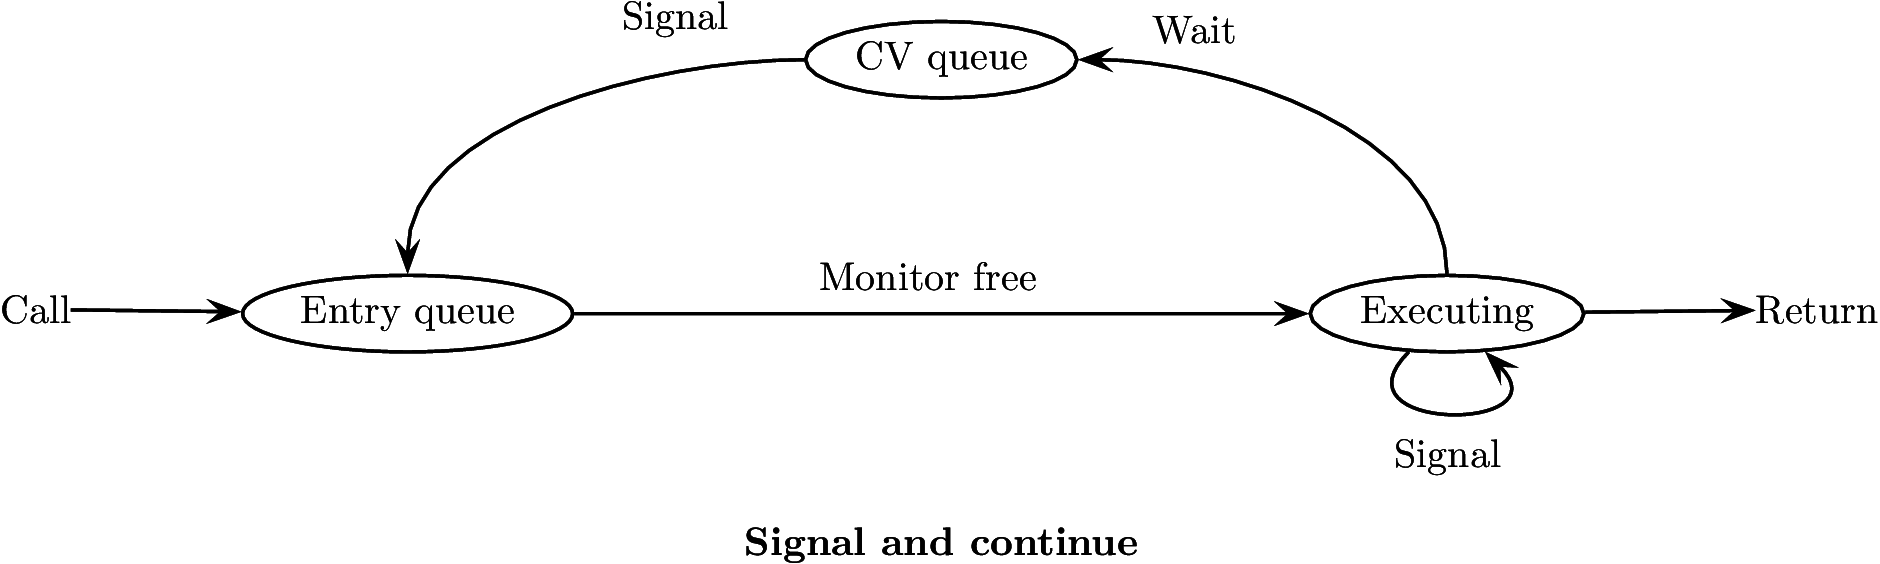
\includegraphics[width=\textwidth]{figures/signalandcontinue.png}
\bi
\ii{The signaler continues and the
signaled process waits.}
\ii{Nonpreemptive.}
\ei
\newpage

\ti{Signal and Wait} 

\bigskip

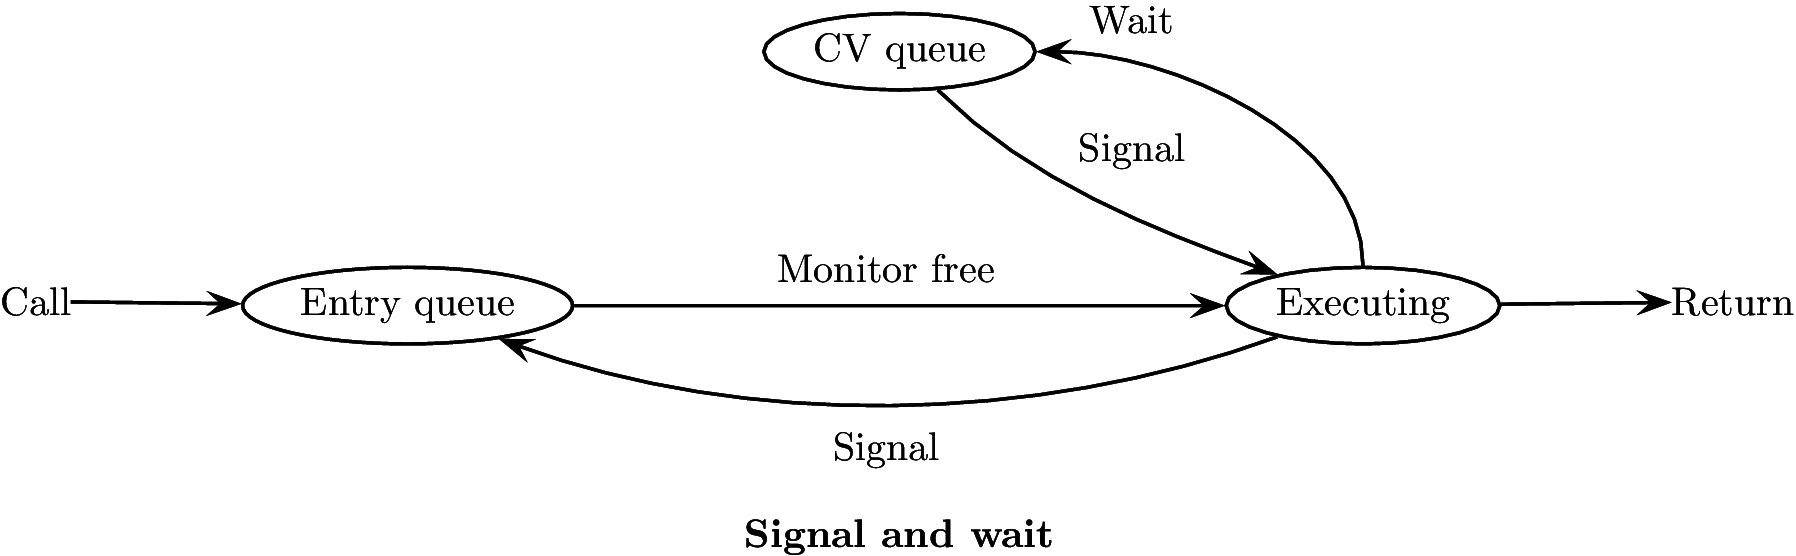
\includegraphics[width=\textwidth]{figures/signalandwait.png}

\bi
\ii{The signaler waits
and the signaled process executes now.}
\ii{Preemptive.}
\ei
\newpage

\myfig{chap05/5_01.pdf}
\myput{60}{Signal and continue used in Java and Pthreads.}
\myput{57}{If signaled process put at front of entry queue: }
\myputn{55}{\bf signal and urgent wait}
\myfigend


\myfig{chap05/5_02.pdf}
\myput{57}{Works for both SC and SW.}
\myput{54}{SW is FIFO, but not SC.}
\myput{51}{With SW, {\tt while} can be replaced by {\tt if}}
\myfigend

\myfig{chap05/5_03.pdf}
\myfigend

\ti{Differences between {\tt P} and {\tt V} and {\tt wait} and {\tt
    signal}}
\bi
\ii {\tt wait} and {\tt P}:
\bi
\ii {\tt wait} {\em always} delays until a {\tt signal}
\ii {\tt P} delays only if semaphore is zero
\ei
\ii {\tt signal} and {\tt V}:
\bi
\ii {\tt signal} has no effect on an empty queue
\ii {\tt V} either awakens a process or increments the semaphore
\ei
\ei

\ti{Book assumes Signal and Continue}
\bi
\ii SC used in Unix, Java, and Pthreads.
\ii Makes {\tt signal\_all} well-defined.
\ii It is compatible with priority-based scheduling.
\ii It has simpler formal semantics.
\ii Historically, SW was first proposed for use in monitors.
\ei


\myfig{chap05/5_04.pdf}
\myfigend
\myfig{chap05/5_05.pdf}
\myfigend
\myfig{chap05/5_06.pdf}
\myfigend
\myfig{chap05/5_07.pdf}
\myfigend
\myfig{chap05/5_08.pdf}
\myfigend
\myfig{chap05/5_09.pdf}
\myfigend
\myfig{chap05/5_10.pdf}
\myfigend

\ti{Skipping disk scheduler \S5.3...except}

\bigskip

\centerline{\Huge {\em Open} and {\em Closed} monitors }
\bi
\ii When a procedure in one monitor calls a procedure in a different monitor:
\bi
\ii If it releases the original monitor it is an {\em open} call.
\ii If it retains the lock on the original monitor it is a {\em closed} call.
\ei
\ei
\newpage
\nop{
\myfig{chap05/5_11.pdf}
\myfigend
\myfig{chap05/5_12.pdf}
\myfigend
\myfig{chap05/5_13.pdf}
\myfigend
\myfig{chap05/5_14.pdf}
\myfigend
\myfig{chap05/5_15.pdf}
\myfigend
\myfigs{1.1}{chap05/5_16.pdf}
\myfigend
\myfig{chap05/5_17.pdf}
\myfigend
\myfig{chap05/p236_Disk_Access.pdf}
\myfigend
}

\ti{Java:  synchronized methods}

\begin{Verbatim}
  class Counter \{
    private int c = 0;
    public void increment() \{
      c++;
    \}
    public int value() \{
      return c;
    \}
  \}
  
  class SynchronizedCounter \{
    private int c = 0;
    public synchronized void increment() \{
      c++;
    \}
    public synchronized int value() \{
      return c;
    \}
  \}
\end{Verbatim}
\newpage

\ti{Java: {\tt wait} and {\tt notify}}

\bi
\ii Methods of the class {\tt Object}
\ii Can only be used in {\tt synchronized} methods
\ii Only a single delay queue per object
\ii There are no condition variables
\bi\ii exactly one (implied) condition variable per object\ei
\ii FIFO not guaranteed
\ii {\tt notifyAll}
\ii Nested calls are closed calls
\ei
\newpage


\myfigs{1}{chap05/p241_Java_rw_parallel.pdf}
\myfigend
\myfig{chap05/p244_Java_rw_exclusive.pdf}
\myfigend
\myfig{chap05/p245_Java_rw_true.pdf}
\myfigend

\ti{Pthreads: locks and condition variables}

\begin{multicols}{2}
\begin{Verbatim}[label=Lock]
...
pthread_mutex_t mutex;
...
pthread_mutex_init(&mutex, NULL);
...
\end{Verbatim}

\begin{Verbatim}[label=Condition variable]
...
pthread_cond_t cv;
...
pthread_cond_init(&cv, NULL);
...
\end{Verbatim}
\end{multicols}

\begin{multicols}{2}
\begin{Verbatim}[label=Thread 0]
...
pthread_mutex_lock(&mutex);
...
pthread_cond_wait(&cv, &mutex);
...
pthread_mutex_unlock(&mutex);
\end{Verbatim}
\begin{Verbatim}[label=Thread 1]
...
pthread_mutex_lock(&mutex);
...
pthread_cond_signal(&cv);
...
pthread_mutex_unlock(&mutex);
\end{Verbatim}
\end{multicols}


\newpage
\myfigsp{.9}{1}{chap05/5_18.pdf}
\myfigend
\myfigsp{.9}{2}{chap05/5_18.pdf}
\myfigend
\end{document}
